% This document is a playground for testing new commands before inserting them
% into the .sty file

\documentclass{scrartcl}

\usepackage{lilyglyphs}

%%%%%%%%%%%%%%%%%%%%%%%%
% Numbers and Dynamics %
%%%%%%%%%%%%%%%%%%%%%%%%

%\newcommand{\lilyNumber}[2][1.35]{\lilyText[#1]{#2}}




\begin{document}

\lilyGlyphByNumber{33} and space?

\lilyRFZ and space

\lilyDynamics{rfz} and space

\section*{Accidentals}
New \sharp accidental \sharpArrowdown and \sharpArrowdown*.\\
New \sharp accidental \sharpArrowup and \sharpArrowup*.\\
New \sharp accidental te \sharpArrowboth and \sharpArrowboth*.
New accidental \sharpSlashslashStem and \sharpSlashslashStem*,.\\
New accidental \sharpSlashslashslashStemstem and \sharpSlashslashslashStemstem*,.\\
New accidental \sharpSlashslashslashStem and \sharpSlashslashslashStem*,.\\
New accidental \sharpSlashslashStemstemstem and \sharpSlashslashStemstemstem*,.\\

\section*{Time Signatures}
	This is a normal Time signature: \lilyTimeSignature{3}{4}.
	
	As the plus sign is also directly accessible you can even
	write \lilyTimeSignature{3\,+\,7}{8+4} easily :-)


	
\section*{PGF/tikz}

Absatz, zusammen mit einem Notenkopf: 
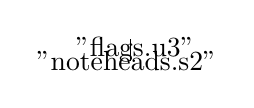
\begin{tikzpicture}
	\draw (0,0) node {\lilyGlyph{"noteheads.s2"}};
	\draw[semithick] (0.3ex,0) -- (0.3ex,0.8em);
	\draw (0.7ex,1ex) node {\lilyGlyph{"flags.u3"}};
\end{tikzpicture}

\Large
Neuer Absatz, zusammen mit einem Notenkopf: 
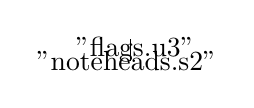
\begin{tikzpicture}
	\draw (0,0) node {\lilyGlyph{"noteheads.s2"}};
	\draw[semithick] (0.3ex,0) -- (0.3ex,0.8em);
	\draw (0.7ex,1ex) node {\lilyGlyph{"flags.u3"}};
\end{tikzpicture}

\normalsize
Neuer Absatz, zusammen mit einem Notenkopf: 
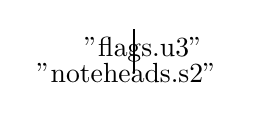
\begin{tikzpicture}[scale=2]
	\draw (0,0) node {\lilyGlyph{"noteheads.s2"}};
	\draw[semithick] (0.3ex,0) -- (0.3ex,0.8em);
	\draw (0.7ex,1ex) node {\lilyGlyph{"flags.u3"}};
\end{tikzpicture}

One sees: It is principally possible to combine graphical and textual elements with pgf/tikz,
but we definitely have to work on it some more: Especially it isn't scalable so far (explicitely or implicitely following text size)
	write \lilyTimeSignature{3+7}{8+4} easily :-)
	
	One more option: \lilyTimeSignature{3}{8} \lilyText{+} \lilyTimeSignature{7}{4}. (note the space that the formula environment makes around it. Maybe this isn't the best approach?

	%\lilyNumber
	
\section*{PGF/tikz}

Absatz, zusammen mit einem Notenkopf: 
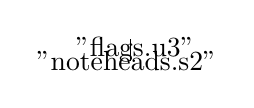
\begin{tikzpicture}
	\draw (0,0) node {\lilyGlyph{"noteheads.s2"}};
	\draw[semithick] (0.3ex,0) -- (0.3ex,0.8em);
	\draw (0.7ex,1ex) node {\lilyGlyph{"flags.u3"}};
\end{tikzpicture}

\Large
Neuer Absatz, zusammen mit einem Notenkopf: 
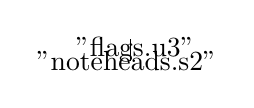
\begin{tikzpicture}
	\draw (0,0) node {\lilyGlyph{"noteheads.s2"}};
	\draw[semithick] (0.3ex,0) -- (0.3ex,0.8em);
	\draw (0.7ex,1ex) node {\lilyGlyph{"flags.u3"}};
\end{tikzpicture}

\normalsize
Neuer Absatz, zusammen mit einem Notenkopf: 
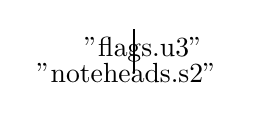
\begin{tikzpicture}[scale=2]
	\draw (0,0) node {\lilyGlyph{"noteheads.s2"}};
	\draw[semithick] (0.3ex,0) -- (0.3ex,0.8em);
	\draw (0.7ex,1ex) node {\lilyGlyph{"flags.u3"}};
\end{tikzpicture}

One sees: It is principally possible to combine graphical and textual elements with pgf/tikz,
but we definitely have to work on it some more: Especially it isn't scalable so far (explicitely or implicitely following text size)

\section*{exchange starred?}

If I write a \flat in a sentence, it is like I expect it.\\
And a \lilyRFZ is equally \lilyRF.

And a time signature \lilyTimeSignature{3}{4}?

A \lilyRFZ in text and at the end \lilyRFZ*.

General Dynamics \lilyDynamics{ff} aren't a problem \lilyDynamics{ff}.


	
>>>>>>> master
\end{document}